% Template for ICIP-2015 paper; to be used with:
%          spconf.sty  - ICASSP/ICIP LaTeX style file, and
%          IEEEbib.bst - IEEE bibliography style file.
% --------------------------------------------------------------------------
\documentclass{article}
\usepackage{spconf,amsmath,graphicx}

% Example definitions.
% --------------------
\def\x{{\mathbf x}}
\def\L{{\cal L}}

% Title.
% ------
\title{Geometric Based Convolutional Neural Networks for Effective\\
 Indoor Scene Layout Estimation}
%
% Single address.
% ---------------
\name{Juntao Feng, Xuejin Chen\thanks{Thanks to XYZ agency for funding.}}
\address{University of Science and Technology of China, Hefei Anhui, China.}
%
% For example:
% ------------
%\address{School\\
%	Department\\
%	Address}
%
% Two addresses (uncomment and modify for two-address case).
% ----------------------------------------------------------
%\twoauthors
%  {A. Author-one, B. Author-two\sthanks{Thanks to XYZ agency for funding.}}
%	{School A-B\\
%	Department A-B\\
%	Address A-B}
%  {C. Author-three, D. Author-four\sthanks{The fourth author performed the work
%	while at ...}}
%	{School C-D\\
%	Department C-D\\
%	Address C-D}
%
\begin{document}
%\ninept
%
\maketitle
%
\begin{abstract}
Layout estimation from a single RGB image is a fundamental and indispensable problem for indoor scene understanding, which models the inner space as a 3D cuboid, including floor, ceiling and walls and their boundaries. However, it is significantly challenging to extract layout structure with large clutter and occlusions.
In this paper, we propose a geometric based networks for a single RGB image which encodes depth and normal information from image itself. We have demonstrated that using geometric information jointly works better than using only RGB images for indoor scene layout estimation with fully convolutional neural networks(FCNN). Then an optimization framework takes full advantages of spacial labelling results and layout boundary relations from networks to generate final layout estimates. The proposed method has proven to achieve competitive accuracy of layout estimation on two commonly used benchmark datasets.
\end{abstract}
%
\begin{keywords}
   Scene understanding, layout estimation, geometric embedding.
\end{keywords}
%


\section{INTRODUCTION}
\label{sec:intro}
The main purpose of indoor scene layout estimation is to extract semantic boundaries among walls, ceiling and floor, and to obtain different planes which provide strong spacial expression of the scene, for cluttered indoor scenes from a single RGB image, as shown in Fig. \ref{fig:definition}. 


\begin{figure}[!ht]
	\centering
	\textsc{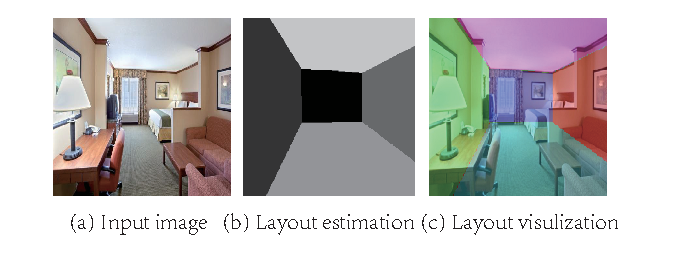
\includegraphics[width=3.5in]{figure/definition.eps}}
	\caption{Examples of indoor scene images. (a) Input images. (b) Layout estimation with semantic labels. (c) Layout visulization superimposed on the input image.}
	\label{fig:definition}
\end{figure}


Layout estimation is a fundamental and indispensable problem for indoor scene understanding, and it plays a critical role in a diverse range of hot applications, such as scene reconstruction, robot navigation, virtual reality, and so on. Moreover, on the Large-scale Scene Understanding Challenge(LSUN), indoor scene layout estimation has become one of the popular tasks towards scene-centric challenges. However, the most important clues such as room corners and layout boundaries are often occluded by a large amount of clutter occuring everywhere in daily life(see Fig.\ref{fig:pipeline} (a)), which make the layout task tough to estimate. Moreover,  illumination variations existed in indoor scene(see Fig.\ref{fig:pipeline} (b-c)), may increase the difficulty of visual understanding. Last but not the least, the views of indoor scene images are in a wide range(see Fig.\ref{fig:pipeline} (d-f)), and such factor can  cause appearance diversity for an indoor scene image.


\begin{figure}[!ht]
	\centering
	\textsc{\includegraphics[width=3.5in]{figure/case.eps}}
	\caption{Examples of indoor scene images. (a) Much clutter. (b) Too bright. (c) Too dark. (d-f) Different views.}
	\label{fig:case}
\end{figure}

\cxj{Related work: from estimation using vanishing points/low-level features, then two-step (FCN+post-processing), to end-to-end network. }
%%
In recent decades, many researchers have made massive attempts to estimate spacial layout from a single image automatically. One popular framework using a 3D cuboid to approximately express indoor scene layout was introduced by \cite{hedau2009recovering} in 2009. The author generated several layout candidates by using vanish point detection. Then it gathered mid-level features like the line membership features and the geometric context features for each candidate and ranked them by using a structured SVM. Unfortunately, the process of layout candidiate generation is highly sensitive and fragile towards a large amount of clutter. Based on this milestone work, several strategies focused on layout hypothesis generation and ranking were considered. Wang et al.\cite{wang2013discriminative} introduced latent variables to model indoor clttuer. Moreover, in \cite{schwing2012efficient}\cite{schwing2013box}, Schwing et al. modeled cllutterd indoor scenes with higher-order potentials and jointly generated layout and objects with box shapes. Some researchers introduced low-level information as geometric restrictions as supplementary in indoor scene problem. Lee et al.\cite{lee2009geometric}. proposed several physically valid structure hypotheses by geometric reasoning and verified to find the best fitting model to line segments. Ramalingam et al.\cite{ramalingam2013manhattan} employed Manhattan Junction grouping to select best layout. As mentioned above, traditional methods need to design image features manually, which greatly increase the complexity and are weekly capable of adapting to dealing with all complex indoor scenes. Besides, there exists a large time consuming for layout candidate generation, which is stongly against our intention to rely on computers to understand the room layout as fastly as possible.

Since the development of the 3D-data capture devices like kinects and RGBD depth cameras, more and more 3D-based methods towards indoor scene field have been studied. Moreover, some researches using 3D-based methods for indoor layout estimation have been studied. Geiger et al.\cite{geiger2015joint} proposed a high-order graphical model and jointly reasoned about the layout, objects and superpixels from RGBD image. Ren et al.\cite{ren2016three} proposed a cloud of oriented gradient descriptor and “Manhattan voxel” that links the 2D appearance and 3D pose of object categories to better capture the 3D room layout geometry and object detection. Guo et al.\cite{guo2015predicting} interpreted layout and 3D model jointly from a RGBD image by aligning to 3D model dataset. 3D information provide additional geometric cues based on planes and objects, which merge big planes and obejects together and weaken the effects of light and complex textures, and thus lead to robust semantic understanding. With 3D-based methods, not only can layout estimation work turn out to be more robust, but also more problems we can solve even 3D modeling  problem for whole indoor scenes.  

Recently, the deep learning methods and convolution neural network(CNN) have achived impressive progresses in various computer vision tasks, such as semantic segmentation \cite{long2015fully}\cite{chen2016deeplab}, object detection \cite{girshick2015fast}\cite{ren2015faster}, scene understanding \cite{gupta2015indoor}\cite{badrinarayanan2017segnet}, and so on. Towards layout estimation problem, several researchers have achieved to adopt deep learning methods to solve it. Mallya et al.\cite{mallya2015learning}, presented a Fully Convolutional Networks (FCNs)\cite{long2015fully} framwork for learning informative edge maps from a single image, which provided as a new information to sample vanishing lines for layout candidates generation and ranking. This work is the first to train CNN to produce robust features used to replace hand-crafted features towards layout estimation problem. However, in the framwork of layout candidates generation and ranking, their algorithm still remained time-consuming. Dasgupta et al.\cite{dasgupta2016delay} used the FCN to learn semantic surface labels including left wall, front wall, right wall, ceiling, and ground. Initial layout generation and optimization were all based on suface belif labels. Unfortunately, Their algorithm relies entirely on FCN's precision for semantic surface labels. In other words, if FCN result gains two much error, we may get totally wrong prediction. Moreover, optimization procedure does not utilize any restrictions based on edge information, just taking random combinations of edges instead, which is geometric inconformity compared with RGB images. Ren et al.\cite{ren2016coarse} adopted a multi-task fully convolutional neural network (MFCN) to jointly predict the room edges and semantic labels. Then a coarse-to-fine method was adopted which enforced several constraints such as layout contour straightness, surface smoothness and geometric constraints to generate fine layout from coarse prediction of room edges. They have considerd geometric constraints to predict high quality estimation results. They need complex geometric computation and rules to generate useful critical lines, however, such low-level features are exactly what we avoid to extract. Zhang et al.\cite{zhang2016learning} used another deconvolution network which has multi-layer deconvolution and a receptive field as large as the entire image compared to FCN. As the result, they can obtain highly reliable edge maps. Then they follow the framework of layout candidates generation using vanish line samplling with an adaptive line sample strategy for robustness and time reduction. A measurement of similarity is proposed between edge map and layout candidates for ranking. Unexpectedly, their results are less precise compared with \cite{dasgupta2016delay}\cite{ren2016coarse}. One explanation may be that the latter two optimization strategies are more effective compared to vanish line sampling.

\cxj{compared to \cite{ren2016coarse}, what is our advantage? They apply geometric constraints as an optimization problem. \cite{dasgupta2016delay} also apply a post-processing step to enforce geometric constraints. One big disadvantage of the post-processing is that it takes seconds to optimize the layout. \cite{dasgupta2016delay} requires 30 seconds for the layout optimization.}\\
\drf{compared to \cite{ren2016coarse}, we have better performance on layout estimation before optimization. ie. the output of our FCN-MC are more reliable because we apply additional information(depth and normals). We use the same post-processing step in \cite{dasgupta2016delay}, so we have the same problem, or maybe worse.}

\cxj{\cite{LeeRoomNet17} presents an end-to-end trainable network that predicts the layout corners and room type A RNNN framework is employed to refine the layout. Different from previous pixel-based representation of the layout, they use a keypoint-based representation.  }

In this work, our algorithm is based on framework of \cite{dasgupta2016delay}, which does not need to extract low features of lines and vanish points from a single RGB image. To enhance the existed FCN's ability, we use networks to estimate depth and normal information from one single RGB image. Then depth and normal information serves as geomtric embedded into FCN networks to jointly generate high quality suface maps and edge maps. Based on\cite{dasgupta2016delay} optimization framwork, we introduce more geometric constraints from predicted edge maps to optimize surface labels to generate high quality layout estimation. Experimental results demonstrate that our method is robust and effective for layout estimation even facing a high clutter on two popular room layout benchmark datasets.
 
 




	
	


%\section{RELATEDWORK}
\label{sec:Rel}

Layout estimation of interior scenes has been drawn substantial attention in computer vision, especially in recent several decades. 
%
According to the methodologies used to recover the layout or structure, we mainly discuss two categories of layout estimation methods: geometric reasoning based on geometric constraints like vanishing points, and neural network-based methods in recent five years. 

%Geometric constraints 
%%%%%%%%%%%%%%%%%%%%%% Single RGB image %%%%%%%%%%%%%%%%%%%%%%%
%
Most of existing approaches recover the scene structure from a single image under the Manhattan world assumption, under which most objects are aligned with three dominant orthogonal directions. 
%
Under this assumption, a three-step pipeline is widely used: vanishing points are estimated from detected line segments, layout hypotheses are created, and then each hypothesis is evaluated according various evidences in the image to find the best one. 
%
\cxj{list each method..}\drf{\cite{hedau2009recovering,wang2013discriminative,mallya2015learning,gupta2010estimating,hedau2010thinking}}
%
More detailed building models are created from line segments in \cite{lee2009geometric} where they consider corner types, edge orientations, and geometric relationships in hypothesis evaluation. 
%drawbacks 
However, these methods usually spend several minutes on the hypothesis evaluation while there are huge number of hypotheses in a cluttered scene. 

%%%%%%%%%%%%%%%%%% BOx in Box %%%%%%%%%%%%%%%%%%%%%%%%%%%%5
Besides of recovering the main wall-floor structure, more geometric inference of objects in the scene are added to generate more accurate estimation in cluttered scenes. 
\cite{hedau2009recovering} reply on cuboid representations to .., while \cite{geiger2015joint} employs more precise 3D models to represent objects, taking the advantage of the depth information. 
%


%
First, only use vanishing lines to generate hypotheses.
Then, add surface orientation constraints. 
Finally, add analysis on the clutter objects or occluding objects in the scene.


%%%%%%%%%%% RGBD image analysis %%%%%%%%%%%%%%%%%%%%%%%%%55
With the development of depth camera, a large number of methods for structure recovery from RGBD images appeared. 
%
\cite{geiger2015joint} jointly infers 3D objects and the scene layout from a single RGBD image via a high-order CRF model.  
%
A novel representation called Manhattan voxel is proposed in \cite{ren2016three} to capture more detailed 3D room layout. 
By employing a cascade of classifiers, the contextual relationships among object categories and scene layout are considered to improve the accuracy of both object categorization and layout estimation. 
% a cloud of oriented gradient descriptor to model perspective project affects for object categorization. 
However, more complicated models brings higher time costs varying from 10 to 30 minutes to analyze a single RGBD image. 


%Deep learning methods 
Deep learning methods and convolution neural network(CNN) have achieved impressive progresses in various computer vision tasks, such as semantic segmentation \cite{long2015fully,chen2016deeplab}, object detection \cite{girshick2015fast,ren2015faster}, scene understanding \cite{gupta2015indoor,badrinarayanan2017segnet}, and so on.
%
Towards the layout estimation problem, Mallya et al.\cite{mallya2015learning} presented a fully convolutional networks (FCNs) framework for learning informative edge maps from a single image, to provide additional hints for sampling vanishing lines for layout candidates generation and ranking. 
%
This work firstly uses CNN to produce robust features instead of hand-crafted features for layout estimation problem. However, the layout hypothesis generation and ranking parts still play as post-processing steps, costing much time as traditional methods. 
%
Dasgupta et al.~\cite{dasgupta2016delay} use FCN to learn semantic surface labels including left wall, front wall, right wall, ceiling, and ground. 
Initial layout generation and optimization were all based on surface belief labels. 
Unfortunately, Their algorithm relies entirely on FCN's precision for semantic surface labels. 
%In other words, if FCN resulting gains two much error, we may get totally wrong prediction.
%
Moreover, the optimization procedure does not utilize any restrictions based on edge information, just taking random combinations of edges instead, which is geometric inconformity compared with RGB images. 
%
Ren et al.~\cite{ren2016coarse} adopted a multi-task fully convolutional neural network (MFCN) to jointly predict the room edges and semantic labels. 
Then a coarse-to-fine method was adopted which enforced several constraints such as layout contour straightness, surface smoothness and geometric constraints to generate fine layout from coarse prediction of room edges. 
%
They have considered geometric constraints to predict high quality estimation results. They need complex geometric computation and rules to generate useful critical lines, however, such low-level features are exactly what we avoid to extract. 
%
Zhang et al.\cite{zhang2016learning} used another deconvolution network which has multi-layer deconvolution and a receptive field as large as the entire image compared to FCN. As the result, they can obtain highly reliable edge maps. Then they follow the framework of layout candidates generation using vanishing line sampling with an adaptive line sample strategy for robustness and time reduction. A measurement of similarity is proposed between edge map and layout candidates for ranking. 
Unexpectedly, their results are less precise compared with \cite{dasgupta2016delay,ren2016coarse}. 
One explanation may be that the latter two optimization strategies are more effective compared to vanish line sampling.
%
\cxj{in comparison, we provide .. }

\section{Our Method}
\label{sec:Meth}


\subsection{System Overview}
\label{subsection:overview}

\begin{figure}[!ht]
	\centering
	\includegraphics[width=3.4in]{figure/pipeline.eps}
	\caption{An overview of our layout estimation algorithm pipeline. First we adopt a multi-scale CNN achitecture to predict geometric information from RGB image, including depth and normals. Then we encode abovementioned information into FCNN , which help to accurately estimate the layout. Optimization framwork based on perspective projection restriction is adopted to generate final precise layout estimates.}
	\label{fig:pipeline}
\end{figure}

Under the Manhattan world assumption, a room layout is represented as cube having at most five walls (Left, Front, Right, Ceiling, Ground) visible in the image. 
%
Given an RGB image $I$ with \cxj{arbitrary?} \drf{yes, but it will be resized to $320\times 240$ and then input into the network~\cite{eigen2015predicting}}size $w\times h$, our algorithm generates a room layout $\vb{L}$ consisting of a surface label for each pixel $L_{ij}\in $ $\{$left wall, front wall, right wall, ceiling, ground$\}$. 
Fig. \ref{fig:pipeline} shows our algorithm pipeline. 
%%step 1
Different from \cite{dasgupta2016delay}, we first estimate the depth depth $D_{I}$ and normal map $N_{I}$ from the input color image to generate \emph{geometric hints} using a multi-scale convolutional architecture~\cite{eigen2015predicting}, as described in Sec.~\ref{sec:depth_normal}.
%step 2
Integrating the original RGB image, the estimated depth and the normal map, a fully convolutional network is used to predict five surface maps, each of which describes the belief for each specific layout surface. Details will be described in Sec.~\ref{sec:surfacelabel}.
%step 3: optimization
To generate more clear and straight boundaries in the final layout, an optimization step is adopted to \cxj{what does this optimzation do?}\drf{The output of the FCN-MC maybe not consistent with the model that we use to parameterize the layout. For example, the boundaries are not straight, there may be multiple disjoint components per label, and it may contain spurious regions like spurious front wall. The optimization do some preprocessing first to prune the extra disjoint components and fill in the hole caused by pruning and judge whether the conbination of the plane is reasonable. Then apply an iterative refinement process to obtain L. So the ultimate goal of the optimization step is to get L which parameterize the straight boundaries of layout.}, as described in Sec.~\ref{sec:optimization}.


\cxj{several questions here }

\begin{enumerate}
	\item \textbf{input image size}: as claimed in \cite{ren2016three}, the receptive field of VGG16 is 404x404, why do we use $321\times 321$?\ \\ \drf{Need to do experiment. As has been revealed by \cite{ren2016three}, if
		the input image size is smaller than the receptive field size, it is padded with zeros and spatial resolution is lost in this case. So $321\times 321$ may be not appropriate, we should change it to $404\times 404$}

\end{enumerate}
 

\comments{
The coarse layout estimation about semantic layout surfaces for a single RGB image, are predicted by fully convolutional neural network with geometric information emmbeded, including depth and normal information. These geometric information are estimated from source RGB image by a multi-scale convolutional architecture\cite{eigen2015predicting}. This will be decribied in Sec. \ref{subsection:CNN}. Then based on optimization framwork proposed in \cite{dasgupta2016delay}, which mainly uses perspective projection constraints, we can obtain final precise layout estimation results.
%
}
\cxj{Figure 3 is very similar with \cite{dasgupta2016delay}..}
 


\subsection{Geometric Fusion FCNN for Coarse Layout Estimation}
\label{sec:depth_normal}

We use the multi-scale convolutional network proposed in \cite{eigen2015predicting} to estimate the depth and normal map from a single RGB image, as Figure~\ref{fig:depthandnormal} shows. 
%
\cxj{More analysis on the results of depth map and normal map.}


\begin{figure}
	\centering
	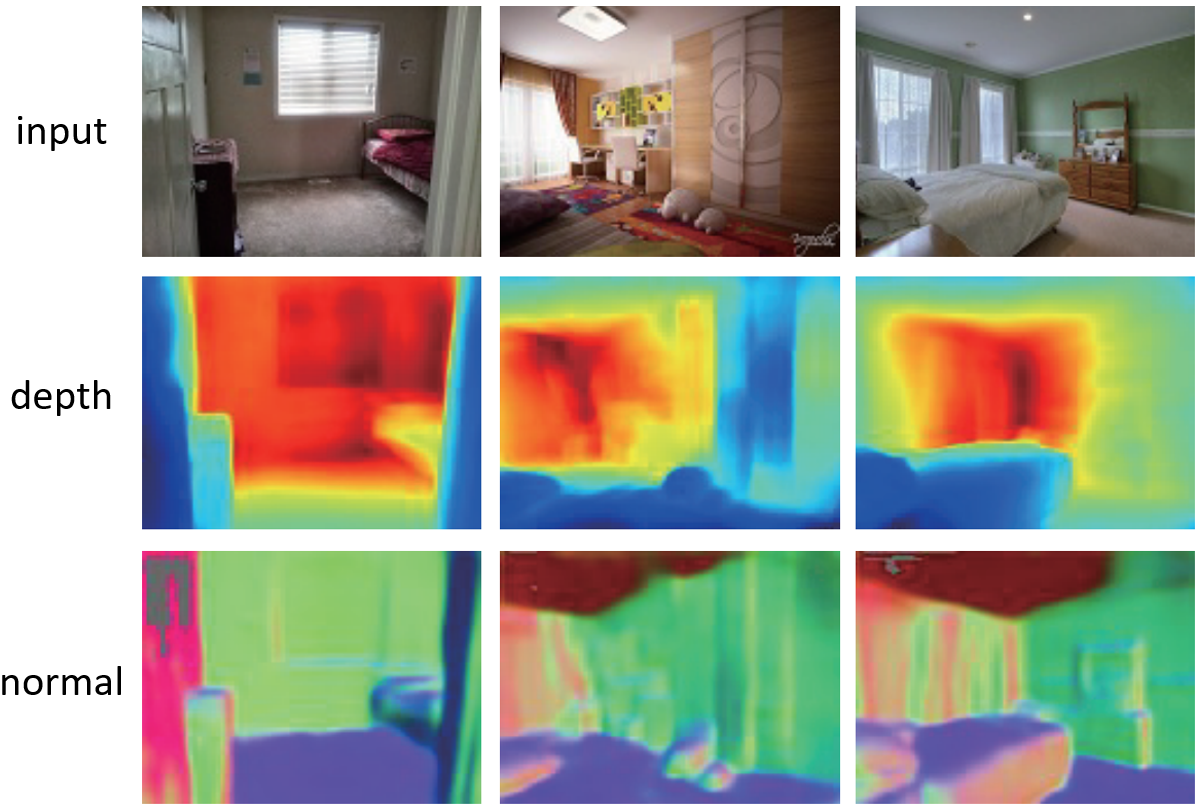
\includegraphics[width=\columnwidth]{figure/geometricinfo1.png}
	\caption{Estimation of depth and normal from a single RGB image using the multi-task FCN in \cite{eigen2015predicting}.}
	\label{fig:depthandnormal}
\end{figure}

\mdf{Though the predicted depth and normal are not accurate}, they provide valuable 3D information for high-level structure estimation, especially in cluttered scenes.
%
Normals can serve as clues tending to merge big planes together, with interference factors like clutter, textures and illumination eliminated to varying degrees. 
%
These mid-level geometric information can be used to adapt and improve performance for layout estimation compared to using RGB only. 



\subsection{Surface Label Prediction using MFCN}
\label{sec:surfacelabel}
%
In previous work, \cite{dasgupta2016delay,ren2016coarse} achieved to use fully convolutional neural network(FCNN) or multi-task fully convolutional neural network~(MFCNN) to predict coarse semantic layout surfaces and layout edges. 
%
However, due to much clutter, complex textures and illumination variations existed, semantic surfaces like walls are visually separated in to pieces, making whole surfaces difficult to aggregate together. 
%
Fig.~\ref{fig:fcn-comparison}(b) shows layout estimation results using FCNN architecture for prediction using a general FCN widely used in previous methods \cite{dasgupta2016delay,ren2016coarse}. 
Under the comparison between the predicted results and the ground truth, we can see that due to the environmental effect of indoor scenes, layout results estimated from FCNN are not reliable. 
When there exits clutter right on the boundaries, such critical clues are partially or entirely excluded, and thus we can not tell location of each plane precisely. 
Moreover, an entire plane may be predicted separately into pieces due to clutter lay in the plane.

\textbf{Network Architecture}
\cxj{Explain the network architecture.}
\drf{We use the network architechure proposed by \cite{ren2016coarse} but with only one output branch while \cite{ren2016coarse} is a multi-task FCN and learn both layout and semantic surface. The architechure is based on VGG16, in Fig. We remove the first branch after fc7 and in turn we don't have to use a joint loss. The network is trained specifically for semantic surface segmentation. And we fuse the depth map and the normal map with rgb image as additional geometric information in the network to improve the performance of segmentation.   }

Given the input RGB image and the estimated geometric information including depth and normal, there are several possible ways to integrate them in a network to predict the surface labels. We introduce two architectures here.
We also resize them to $321 \time 321$ as input to the following FCN. 

The first way is treading the depth and normal map as four additional channels associated with the input RGB image. Given the seven-channel input (3 channels from RGB, 1 channel from depths and 3 channels from normals), we train a \mdf{VGG16 FCN} to predict the five belief maps for the five surfaces in a room. The network architecture is shown in Fig.~\ref{fig:fcn-multi-channel}. This architecture is named as FCN-MC in this paper. 
%
However, it is intuitively seen that different channels have a wide range of variance and they probably can not be directly fused at the beginning convolutional layers. 

\begin{figure}
	\centering
	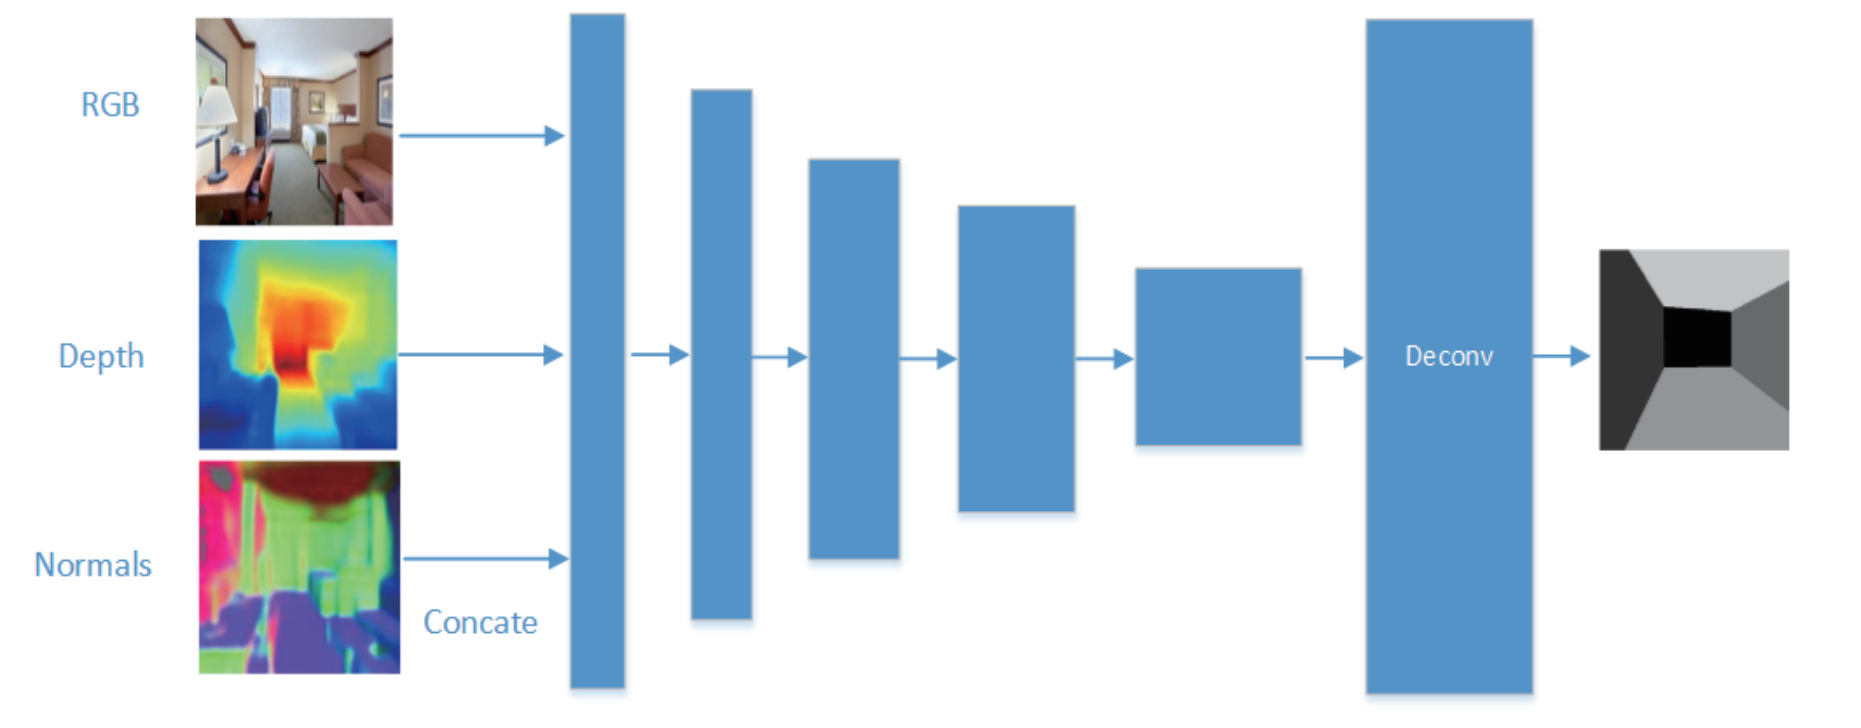
\includegraphics[width=\columnwidth]{figure/fcn-multi-channel.png}
	\caption{A simple network architecture taking the RGB, depth and normal together as input to a VGG16 FCN. \cxj{add more details of each layer.}}
	\label{fig:fcn-multi-channel}
\end{figure}

The second way to integrate them is to later fuse the features that are extracted from different channels separately with a number of convolutional layers. 
This network is named as FCN-GF (geometric fusion), whose architecture is shown in Fig.~\ref{fig:fcn-geometric-fusion}.
  
\begin{figure}
	\centering
	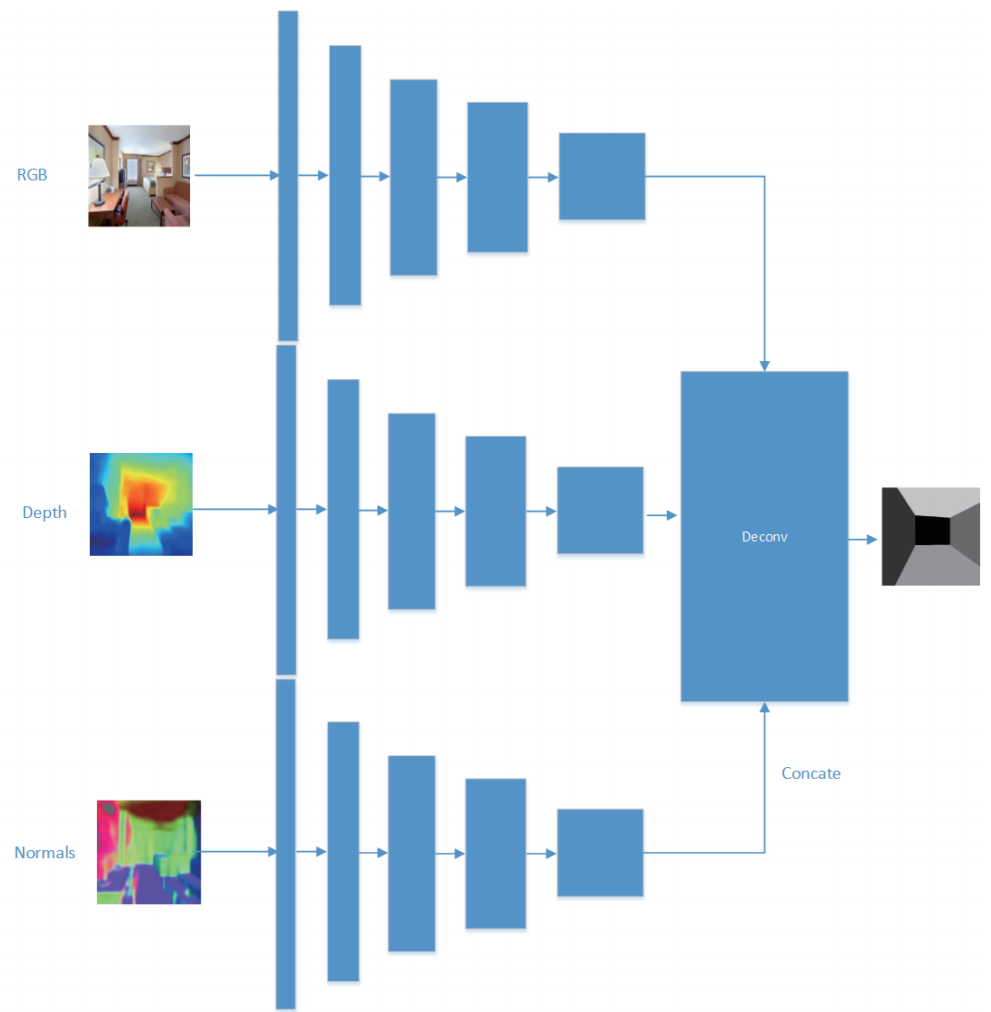
\includegraphics[width=\columnwidth]{figure/fcn-geometric-fusion.png}
	\caption{A network architecture that fuses the RGB, depth and normal together later. \cxj{add more details of each layer.}}
	\label{fig:fcn-geometric-fusion}
\end{figure}


For both networks to predict the five surface maps, the loss function is defined as the softmax ...\cxj{check wiht Fengjuntao. thesis page 18.}
\drf{According to fengjuntao, the loss function was written by himself but probably not standard. I check the softmaxwithloss function on the internet and i think the formulation should be written as...or ...   }
\cxj{The output is five maps or a single map with five surface labels?}
\drf{The output of the FCN-MC/FCN-GF is a $w\times h \times 5$ multidimensional array T, where w and h is the width and length of the input rgb image, and each of the 5 slices can be interpreted as a classification map for a specific label. \\A single map with five surface labels can be obtained by simply picking the label with the highest score for each pixel among those 5 slices. and we use this single map for step3: optimization. }


\textbf{Training}
\cxj{How do you train this network with additional input? Any option to change the network? Do you modified the network parameters? say number of neurons or layers?}
\drf{For FCN-MC, depth map and normals map are merged with the rgb image as new channels and input to the FCN. }

\begin{figure}[!ht]
	\centering 
	\textsc{\includegraphics[width=3.4in]{figure/fcn.eps}}
	\caption{Layout estimation results using different architectures. Row from top to bottom: (a) the input RGB image. (b)(c)(d)Surface predictions using the FCNN architecture used in \cite{dasgupta2016delay,ren2016coarse}, our FCN-MC and FCN-GF respectively. (e) The ground truth. }
	\label{fig:fcn-comparison}
\end{figure}

\cxj{Result analysis for different architures. } 
\drf{For FCN-MC, We treat the normal and the depth as homogeneous information of the rgb image and are a supplement to the rgb image. These addtitional information can serve as context constraints to improve the performance of the network.\\For FCN-GF, we treat the normal and the depth as unhomogeneous information of the rgb image and may disrupt the network parameters as they share weights with the rgb image in the following convolution layers during training. So we learn these information sepertately and fuse them in high-level layer. ie. conv5-3. (more detailed result analysis coming soon..)  }
From Table~\ref{table:fcn-accuracy}, we can see that ...\cxj{FCN-GF is better than FCN-MC?}
\drf{We expect that the performance of FCN-GF should be better than FCN-MC, but it turns out that FCN-MC slightly outperforms FCN-GF. Furthermore, the structrue of FCN-MC have less paramters than FCN-GF, so it's time saving and memory saving compared to FCN-MC.\\Although the result reveals FCN-MC is better, the structure of FCN-GF is still worth trying, as the depth maps used as input to the network are not standard. ie. They are encoded to 3 channels rgb images and should be decoded to gray scale image. And the batch size in training stage may be not appropriate due to hardware limitation. }
Our method generate much more clear edges, less holes. 


\begin{table}
	\centering
	\caption{Pixelwise accuracy for surface label prediction.}
	\label{table:fcn-accuracy}
	\begin{tabular}{c|c}
		\hline
	Network & Accuracy\\
	\hline
	FCN-32s & 0.8109 \\ 
	FCN-MC  & 0.8392 \\
	FCN-GF  & 0.8350 \\
		\hline
	\end{tabular}
		
\end{table}



\cxj{Do test on RGBD images...}




\subsection{Layout Generation}
\label{subsection:optimization}
We adopt a popular model that several  researchers~\cite{hedau2009recovering,dasgupta2016delay,ren2016coarse} have been used to parameterize indoor layout based on the Manhattan world assumption. 
Indoor scene layout can be modeled as 

\begin{equation}
	\label{eq:Layout}
	L = (l1, l2, l3, l4, v)
\end{equation}
where $l_{i}$ stands for $i^{th}$ vanishing line and $v$ stands for the specific vanishing point. The whole scene is equivalent to be labeled to five semantic surfaces, coresponding to (front, left, right, ceiling, ground), as described in Fig. \ref{fig:2.model}. Based ob Eq. (\ref{1.Layout}), each surface can be reconstructed with vanishing lines, extension lines between vanishing point and Intersection point, and image boundaries. Due to the camera pose, not five surfaces are always visible, and such layout can still be modeled by Eq. (\ref{1.Layout}). Different examples are given in Fig. \ref{fig:3.example}.
\section{RESULTS}
\label{sec:Res}



Compared with \cite{ren2016three}, our error is 9.51, their error is 9.31. 
\cxj{How about time cost? Is our method faster?}
\drf{need to do some research}


\begin{table}
	\centering 
	\caption{Performance benchmarking on Hedau's dataset}
	\label{table:comparison-hedau}
	\begin{tabular}{l|c}
		\hline 
	Method & Pixel Error (\%) \\
	\hline
	Proposed FCN-GF & xxx \\
		\hline
	\end{tabular}
\end{table}



\begin{table}
	\centering 
	\caption{Performance benchmarking on the LSUN dataset}
	\label{table:comparison-lsun}
	\begin{tabular}{l|c|c}
		\hline 
		Method & Corner Error (\%) & Pixel Error (\%) \\
		\hline
		Hedau et al. (2009)~\cite{hedau2009recovering} & 15.48 & 24.23 \\
		Mallya et al. (2015)~\cite{mallya2015learning} & 11.02 & 16.71 \\
		Dasgupta et al. (2016)~\cite{dasgupta2016delay} & 8.20 & 10.63 \\
		Ren et al. (2016)~\cite{ren2016three} & 7.95 & 9.31 \\
		Proposed FCN-GF & xxx & 9.51 \\
		\hline
	\end{tabular}
\end{table}
\section{CONCLUSION}
\label{sec:Con}

\section{REFERENCES}
\label{sec:ref}

\bibliographystyle{IEEEbib}
\bibliography{refs}

\end{document}
